\chapter{Results}

\section{Optimization Results}

The optimizations listed in this section has been estimated using a $30$ particle Quantum Dot system with a Padé Jastrow Factor.

Profiling the code revealed that, not surprisingly, $~99\%$ of the runtime was spent in the \\\verb+QMC.diffuse_walker+ function for both VMC, DMC and ASGD. Optimizing the code then solely involved optimizing this function. 

The profiling tool of choice was KCacheGrind, aviable at the Ubuntu Software Center. KCacheGrind lists relative time spent in functions graphically in blocks, whose size is proportional to the time spent inside the function, much like standard hard drive listing software does with files and file size.

Prior to the listed optimizations, all other optimizations mentioned in previous sections has been implemented. The reason why they are not explicitly listed is the fact that they were implemented from start, and are considered ``standard optimizations''. Writing a program without them was considered pointless. 

\subsubsection{Storing the Slater Matrix}

This optimization is described in detail in Section \ref{sec:storeSlater}. In addition to storing the slater, the calculation of $\tilde I$ from the Slater inverse updating algorithm in Eq.~(\ref{eq:Itilde}) was pre calculated outside the main loops.

The percentages listed in the following table is the total time spent inside this specific function relative to all other functions. 

\begin{tabular}{ll}
 \verb+Orbitals.phi+ & \\
 \hline\hline
 Relative time spent prior to optimization & 80.88\% \\
 Relative time spent after optimization    & 8.2\% \\
 \hline
 Relative speedup                          & 9.86
\end{tabular}

The speedup is not because of optimizations within the function itself, but rather due to far less calls to the function. If the calculation of $\tilde I$ was done outside the main loops in the first place, the speedup would be far less. 


\subsubsection{Optimized Jastrow Gradient}

The optimization described in this Section is discussed in detail in Section \ref{sec:optJastGrad}.

The percentages listed in the following table is the total time spent inside this specific function relative to all other functions. 

\begin{tabular}{ll}
 \verb+Jastrow.get_grad+ + \verb+Jastrow.calc_dJ+ & \\
 \hline\hline
 Relative time spent prior to optimization & 40\% \\
 Relative time spent after optimization    & 5.24\% \\
 \hline
 Relative speedup                          & 7.63
\end{tabular}

Exploiting the symmetries of the Padé Jastrow Gradient in addition to calculating the new gradient based on the old is in other words extremely efficient. Keep in mind however, that these results are for a high number of particles. For e.g. two particles, this optimization would not matter at all.

\subsubsection{Storing the Orbital Derivatives}

This optimization is covered in detail in Section \ref{sec:storeSlater}. Much like for the Slater matrix, the optimization in this case comes from the fact that the function itself is called fewer times, rather than being optimized.

The percentages listed in the following table is the total time spent inside this specific function relative to all other functions. 


\begin{tabular}{ll}
 \verb+Orbitals.dell_phi+ & \\
 \hline\hline
 Relative time spent prior to optimization & 56.27\% \\
 Relative time spent after optimization    & 7.31\% \\
 \hline
 Relative speedup                          & 7.70
\end{tabular}


\subsubsection{Storing the Quantum Number Independent Terms}

This optimization is covered in detail in Section \ref{sec:optSPWFqnumIndie}. This optimization lowers the number of exponential function calls, and hence optimizes the calculation time of single particle states, its gradients and Laplacians.

The percentages listed in the following table is the total time spent inside this specific function relative to all other functions. 

\begin{tabular}{ll}
 \verb+Jastrow.get_grad+ + \verb+Jastrow.calc_dJ+ & \\
 \hline\hline
 Relative time spent prior to optimization & 5.85\% \\
 Relative time spent after optimization    & 0.13\% \\
 \hline
 Relative speedup                          & 45
\end{tabular}

This result is not surprisingly equal to $15$ quantum numbers (for $30$ particles) times three. One from the orbitals, and two from their gradients. Prior to this optimization, $45$ exponential calls was needed to fill a row in the Slater matrix and the derivative matrix; this has been reduced to one.

\subsubsection{Overall Optimization}

Combining all the optimizations listed in this chapter, the final runtime was reduced to $5\%$ of the original. The final scaling was


\section{Validating the code}

\subsection{Calculation for non-interacting particles}

For non-interacting particles in a Quantum Dot, no Jastrow factor and $\alpha=1$ provides the exact wave function. This serves as a powerful guide, since results can be benchmarked against exact solutions. In the non-interacting case, the minimization should always yield $\alpha=1$.

Let $R$ denote the highest filled \textit{shell}, i.e. the maximum value of $n_x + n_y$, $N_j$ be the number of particles in a given shell ($1\le j\le R$), $\chi$ be the spin levels and $\epsilon_i = i\omega$, where $i=n_x + n_y$, is the single particle energy at shell level $i$. Then the non-interacting energy of a closed shell Quantum Dot is

\begin{align}
 E_0 &= \sum_\chi\sum_{i=1}^R\sum_{j=1}^{N_i} \epsilon_i \\
     &= 2\sum_{i=1}^R N_i i \omega 
\end{align}

Realizing that (not counting spin) $N_i = i$ for a Quantum Dot, we get

\begin{align}
 E_0 &= 2\omega\sum_{i=1}^R i^2 \\
     &= 2\omega \left(\frac{1}{6}R(R+1)(2R + 1)\right) \\
     &= \frac{R}{3}(R + 1)(2R + 1)\omega
\end{align}

which tabulated for the lowest lying shells yields

\begin{center}
 \begin{tabular}{cc|c}
 R & N  & $E_0/\omega$ \\
 \hline
 1 & 2  & 2  \\
 2 & 6  & 10 \\
 3 & 12 & 28 \\
 4 & 20 & 60 \\
 5 & 30 & 110\\
 6 & 42 & 182\\
 \end{tabular}
\end{center}

The first step to validating the code would be to reproduce these exact results. The minimization method should seek an $\alpha$ close to one, where the variational derivative should be zero. In Table \ref{tab:res_valid_qdots}, validation runs for the three lowest shells are run. Figure \ref{fig:ASGD_nonint} shows the ASGD method finding the minima.


\begin{table}
\begin{center}
\begin{tabular}{cc|cccc}
    N     & $\omega$ & $\mathrm{E_{VMC}}$ & $\mathrm{E_{DMC}}$ & $\alpha$ & $E_0$ \\
\hline
    2     &   0.5    &   1.0    &   1.0    &   1.0    & 1 \\
          &   1.0    &   2.0    &   2.0    &   1.0    & 2 \\
    6     &   0.5    &   5.0    &   5.0    &   1.0    & 5 \\
          &   1.0    &   10.0   &   10.0   &   1.0    & 10 \\
    12    &   0.5    &   14.0   &   14.0   &   1.0    & 14 \\
          &   1.0    &   28.0   &   28.0   &   1.0    & 28 \\
\end{tabular}
\caption{Validation results for Quantum Dots generated using 2000 to 3000 ASGD cycles starting from $\alpha=0.5$. The sampled variance from DMC and VMC is of order $10^{-16}$ (non-zero due to small deviations in $\alpha$ from unity). The last column lists the exact energies. As required we have an exact match (to machine precision). Hard coding $\alpha=1.0$ will yield zero variance.}
\label{tab:res_valid_qdots}
\end{center}
\end{table}


\begin{figure}
 \begin{center}
  \subfigure{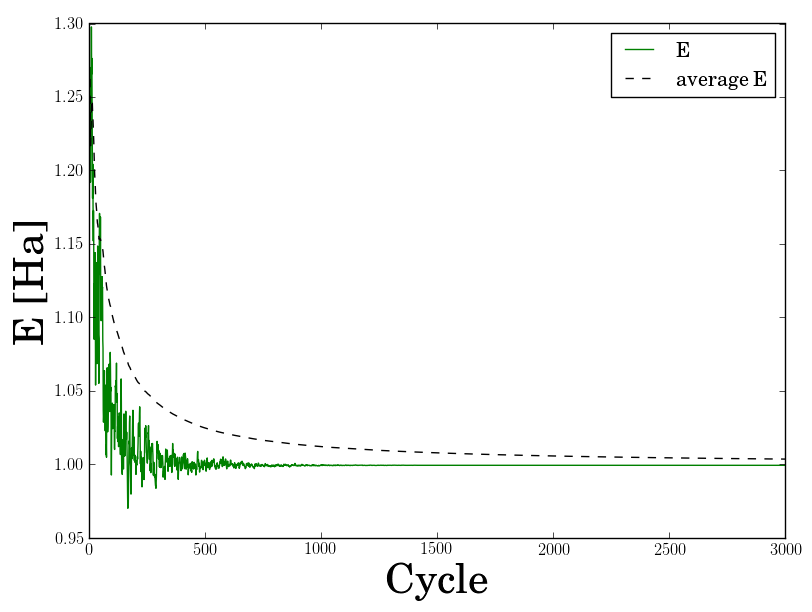
\includegraphics[scale=0.5]{../Graphics/ASGD_nonint_E.png}}
  \subfigure{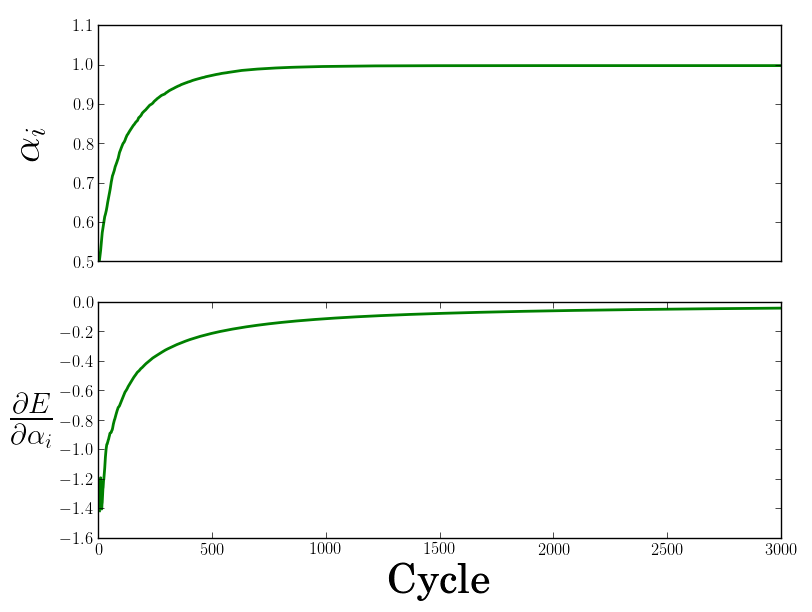
\includegraphics[scale=0.5]{../Graphics/ASGD_nonint.png}} 
  \caption{ASGD results for a non-interaction two-particle Quantum Dot with $\omega=0.5$. The exact energy of $E_0=1$ is reached after approximatly 1000 cycles, where $\alpha$ has converged close to unity. Due to enormous fluctuations, the variational derivative is plotted as an accumulated average, and is in practice dead zero after 1000 cycles. The variational principle described in Section \ref{sec:selectingOptVarPar} is governing the trend of the energy convergence, however, alot of statistical noise is present in the first 1000 cycles due to high variance and few samples.}
  \label{fig:ASGD_nonint}
 \end{center}
\end{figure}

Similar validation can be done for atoms, and is listed in Table \ref{tab:res_valid_atoms}. The non-interaction energy is given by the following expression

\begin{equation}
 E_0 = -\frac{N^2}{2}\sum_{i=1}^N \frac{1}{n_i^2}
\end{equation}


\begin{table}
\begin{center}
\begin{tabular}{c|cccc}
    N     & $\mathrm{E_{VMC}}$ & $\mathrm{E_{DMC}}$ & $\alpha$ & $E_0$\\
\hline
    2     &   -4.0   &   -4.0   &   1.0  & -4  \\
    4     &  -20.0   &  -20.0   &   1.0  & -20 \\
    10    &  -200.0  &  -200.0  &   1.0  & -200\\
\end{tabular}
\caption{Validation results for Atoms generated in a similar way to the Quantum Dots results in Table \ref{tab:res_valid_qdots}.}
\label{tab:res_valid_atoms}
\end{center}
\end{table}

The DMC method in case of an exact wave function should do nothing. The trial energy should equal the ground state energy through all time steps and zero fluctuations in the number of walkers should occur. This trend is shown for Neon in Fig. \ref{fig:DMC_neon_nonint}.

\begin{figure}
 \begin{center}
  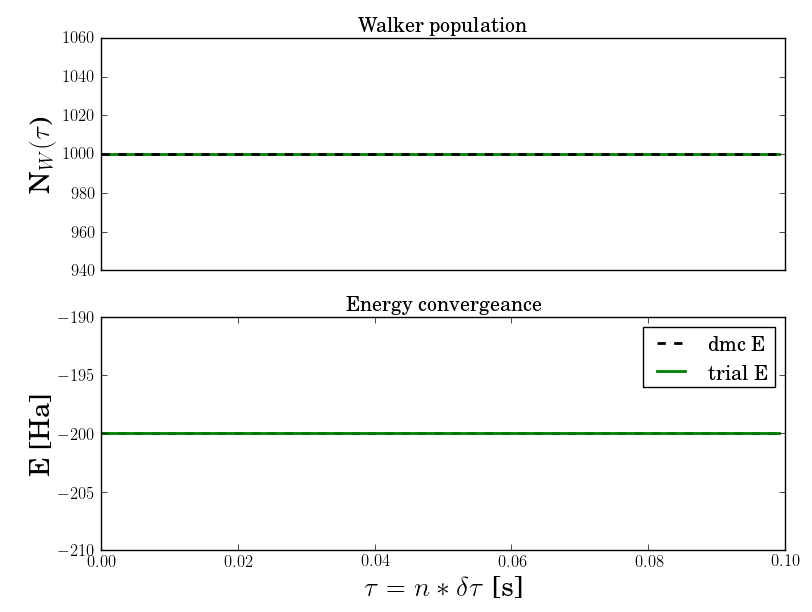
\includegraphics[scale=0.5]{../Graphics/DMC_neon_valid.png}
  \caption{DMC convergence for the Neon result listed in Table \ref{tab:res_valid_atoms}. The trial energy is fixed at the exact ground state energy as expected. The number of walkers are constant, implying a approximatly zero variance.}
  \label{fig:DMC_neon_nonint}
 \end{center}
\end{figure}

A final non-interacting case to run is the case of DMC without the exact wave function. As discussed in Chapter \ref{ch:QMC}, DMC should result in a better estimate of the ground state energy than VMC in case of a trial wave function different from the exact grouns state. A test-case is presented in Fig. \ref{fig:DMC_nonExactWF}.

\begin{figure}
 \begin{center}
  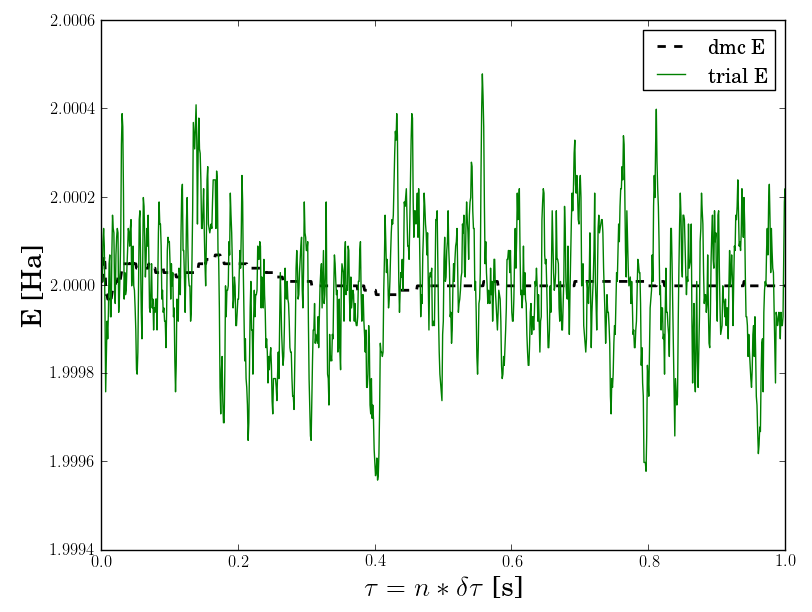
\includegraphics[scale=0.5]{../Graphics/DMC_notExactWF.png}
  \caption{DMC convergence for a non-interacting two-particle Quantum Dot with $\omega=1$. Calculations are done with $\alpha=0.75$, where the exact wave function is given for $\alpha=1$. Unlike the case with the exact wave function, the trial energy oscillates around the exact value. The final result (with blocking) reveals a DMC energy of $2.00000(2)$, where the original VMC energy was $2.0042(3)$. The exact energy is $2.0$ Ha. This illustrates the power of DMC over VMC in the interesting cases with an unknown exact wave function. The calculation were done with $10000$ walkers.}
  \label{fig:DMC_nonExactWF}
 \end{center}
\end{figure}

\section{Results for Quantum Dots}



\begin{table}
\begin{center}
\begin{tabular}{rl|rrrrrr}
    N     & $\omega$ & $\mathrm{E_{VMC}}$ & $\mathrm{E_{DMC}}$ & $E_\mathrm{ref}^{(a)}$& $E_\mathrm{ref}^{(b)}$ & $E_\mathrm{ref}^{(c)}$ & $E_\mathrm{ref}^{(d)}$\\
\hline\hline
\multicolumn{8}{c}{} \\
    2     &   0.1    & 0.44130(5)  & 0.44079(1)   & - 		&- 			& 0.4408 \{23\} & 0.44079191 \{19\}\\
          &   0.28   & 1.02215(5)  & 1.02164(1)   & -		&0.99263 \{19\} 	& 1.0217 \{23\}  & 1.0216441 \{19\}\\
          &   0.5    & 1.66021(5)  & 1.65977(1)   & 1.65975(2)&1.643871 \{19\}	& 1.6599 \{23\}  & 1.6597723 \{19\}\\
          &   1.0    & 3.00030(5)  & 3.00000(1)   & 3.00000(3)&2.9902683 \{19\}	& 3.0002 \{23\}  & 3.0000001 \{19\}\\
\cline{2-8}
\multicolumn{8}{c}{} \\
    6     &   0.1    &  3.5690(3)  &  3.55385(5)  & -		&3.49991 \{18\} 	& 3.5805 \{22\}  & 3.551776 \{9\}\\
          &   0.28   &  7.6216(4)  &  7.60019(6)  & 7.6001(1) &7.56972 \{18\} 	& 7.6254 \{22\}  & 7.599579 \{6\}\\
          &   0.5    & 11.8103(4)  & 11.78484(6)  & 11.7888(2)&11.76228 \{18\}	& 11.8055 \{22\} & 11.785915 \{6\}\\
          &   1.0    & 20.1902(4)  & 20.15932(8)  & 20.1597(2)&20.14393 \{18\}	& 20.1734 \{22\} & 20.160472 \{8\}\\
\cline{2-8}
\multicolumn{8}{c}{} \\
    12    &   0.1    & 12.3162(5)  & 12.26984(8)  & - 		&12.2253 \{17\} 	& 12.3497 \{21\} & 12.850344 \{3\}\\
          &   0.28   & 25.7015(6)  & 25.63577(9)  & - 		&25.61084 \{17\} 	& 25.7095 \{21\} & 26.482570 \{2\}\\
          &   0.5    & 39.2343(6)  & 39.1596(1)   & 39.159(1) &39.13899 \{17\}	& 39.2194 \{21\} & 39.922693 \{2\}\\
          &   1.0    & 65.7905(7)  & 65.7001(1)   & 65.700(1) &65.68304 \{17\}	& 65.7399 \{21\} & 66.076116 \{3\}\\
\cline{2-8}
\multicolumn{8}{c}{} \\
    20    &   0.1    &  30.0729(8)  &  29.9779(1) & -		&29.95345 \{16\}	& 30.2700 \{8\} & 34.204867 \{1\}\\
          &   0.28   &  62.0543(8)  &  61.9268(1) & 61.922(2) &61.91368 \{16\}	& 62.0676 \{20\} & 67.767987 \{1\}\\
          &   0.5    &  94.0236(9)  &  93.8752(1) & 93.867(3) &93.86145 \{16\}	& 93.9889 \{20\} & 100.93607 \{1\}\\
          &   1.0    & 156.062(1)   & 155.8822(1) & 155.868(6)&155.8665 \{16\}	& 155.9569 \{20\}& 164.61280 \{1\}\\
\cline{2-8}
\multicolumn{8}{c}{} \\
    30    &   0.1    &  60.584(1)  &  60.4205(2)  & -		&60.43000 \{15\}	&  61.3827 \{9\}& -\\
          &   0.28   & 124.181(1)  & 123.9683(2)  & - 		&123.9733 \{15\}	& 124.2111 \{9\}& -\\
          &   0.5    & 187.294(1)  & 187.0426(2)  & - 		&187.0408 \{15\}	& 187.2231 \{19\}& -\\
          &   1.0    & 308.858(1)  & 308.5627(2)  & -	 	&308.5536 \{15\}	& 308.6810 \{19\}& -\\
\cline{2-8}
\multicolumn{8}{c}{} \\
    42    &   0.1    & 107.881(1)  & 107.6389(2)  & - 		&- 			& 111.7170 \{8\}& -\\
          &   0.28   & 220.161(1)  & 219.8426(2)  & - 		&219.8836 \{14\}	& 222.1401 \{8\}& -\\
          &   0.5    & 331.002(1)  & 330.6306(2)  & - 		&330.6485 \{14\}	& 331.8901 \{8\}& -\\
          &   1.0    & 544.2(8)    & 542.9428(8)  & - 		&542.9528 \{14\}	& 543.1155 \{18\}& -\\
\hline\hline


\end{tabular}
\caption{Results for Quantum Dots with fixed node approximation calculated on the cluster Abel using $10^8$ VMC cycles, $64000$ walkers, with $2000$ DMC cycles on 128 cores. Ref: $(a)$: F. Pederiva \cite{MagnusArticle} (DMC), $b$: S. Reimann \cite{Sarah} (SRG), $c$: C. Hirth \cite{Hirth} (CCSD), $d$: V. K. B. Olsen \cite{Olsen} (FCI). The numbers inside curly brackets denote the number of shells used above \textit{Fermi-level} to contruct the basis for the calculation.}
\label{tab:QDotsResultsAll}
\end{center}
\end{table}

\section{FIXED NODE TESTS}

\begin{table}
\begin{center}
\begin{tabular}{rl|rrc}
    N     & $\omega$ & $\mathrm{E_{DMC}}$ & $\mathrm{E_{DMC}^\mathrm{F.N.}}$  & $\epsilon_\mathrm{DMC}^\mathrm{F.N.}/\overline{\sigma}$ \\
\hline\hline
\multicolumn{5}{c}{} \\
    2     &   0.1    & 0.44079(1) & 0.44079(1)  & 0 \\
          &   0.28   & 1.02164(1) & 1.02164(1)  & 0 \\
          &   0.5    & 1.65977(1) & 1.65977(1)  & 0 \\
          &   1.0    & 3.00000(1) & 3.00000(1)  & 0 \\
\cline{2-5}
\multicolumn{5}{c}{} \\
    6     &   0.1    &  3.55385(5) & 3.55374(5) & 2.2  \\
          &   0.28   &  7.60019(6) & 7.60016(5) & 0.54 \\ 
          &   0.5    & 11.78484(6) & 11.78489(6)& 0.83 \\
          &   1.0    & 20.15932(8) & 20.15945(7)& 1.73 \\
\cline{2-5}
\multicolumn{5}{c}{} \\
    12    &   0.1    & 12.26984(8) & 12.26986(8)& 0.25\\
          &   0.28   & 25.63577(9) & 25.6358(1) & 0.32 \\
          &   0.5    & 39.1596(1) & 39.1594(1)  & 2 \\
          &   1.0    & 65.7001(1) & 65.7000(1)  & 1 \\
\cline{2-5}
\multicolumn{5}{c}{} \\
    20    &   0.1    &  29.9779(1) & 29.9779(2) & 0 \\
          &   0.28   &  61.9268(1) & 61.9265(2) & 2 \\
          &   0.5    &  93.8752(1) & 93.8752(2) & 0 \\
          &   1.0    & 155.8822(1) & 155.8821(2)& 0.66 \\
\cline{2-5}
\multicolumn{5}{c}{} \\
    30    &   0.1    &  60.4205(2) & 60.4207(2) & 1 \\
          &   0.28   & 123.9683(2) & 123.9682(2)& 0.5 \\
          &   0.5    & 187.0426(2) & 187.0430(2)& 2 \\
          &   1.0    & 308.5627(2) & 308.5626(2)& 0.5 \\
\cline{2-5}
\multicolumn{5}{c}{} \\
    42    &   0.1    & 107.6389(2) & 107.638(2) & 0.81 \\
          &   0.28   & 219.8426(2) & 219.8426(3)& 0 \\
          &   0.5    & 330.6306(2) & 330.6307(2)& 0.5 \\
          &   1.0    & 542.9428(8) &    -       & - \\
\hline\hline
\end{tabular}
\caption{Results for Quantum Dots without fixed node approximation calculated on the cluster Abel using $2000$ DMC cycles on 128 cores. $\epsilon_\mathrm{DMC}^\mathrm{F.N.} = |\mathrm{E_{DMC}} - \mathrm{E_{DMC}^{F.N.}}|$. $\overline{\sigma}  = \frac{1}{2}(\sigma_\mathrm{DMC} + \sigma_\mathrm{DMC}^\mathrm{F.N.})$. The last column serves as an indicator of how many average standard deviations the results differ. For two particles, where the fixed node approximation does not affect the system, the results are as expected exactly the same. For all other system sizes, the difference is mostly within one deviation. This indicates that the effect due to the fixed node approximation for closed shell Quantum Dots are very small.}
\end{center}
\end{table}

